\documentclass[12pt]{article}
\usepackage[left=1in,top=1in,right=1in,bottom=1in]{geometry}
\usepackage{graphicx}
\usepackage{titling}
\usepackage[bookmarks=true,colorlinks=true, linkcolor=red, citecolor=cyan]{hyperref}

\setlength{\droptitle}{-1.0in}   % This is your set screw


\begin{document}


\title{FQL IDE Manual}
\author{Ryan Wisnesky}
\date{\today}

\maketitle

%\begin{abstract}
%This manueal describe FQL IDE to database practitioners without backgrounds in category theory.
%\end{abstract}
\vspace{-0.5in}

\begin{footnotesize}
\tableofcontents
\end{footnotesize}
\newpage

\section{Introduction}

FQL, a {\it functorial query language}, implements {\it functorial data migration}.  Although functorial data migration is formally defined using the language of category theory, it is possible to understand functorial data migration at the level of relational database tables.  Indeed, the FQL compiler emits SQL (technically, PSM) code that can be run on any RDBMS.  The FQL compiler is hosted inside of an integrated development environment, the FQL IDE.  The FQL IDE is an open-source java program that provides a code editor for and visual representation of FQL programs.  A screen shot of the initial screen of the FQL IDE is shown below.

\begin{center}
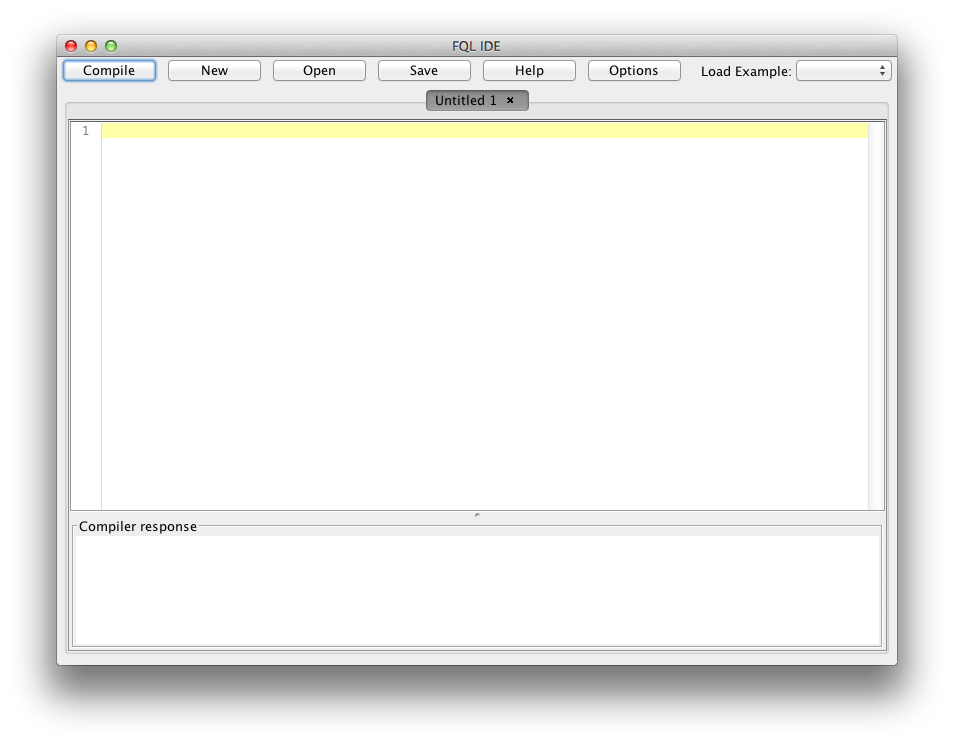
\includegraphics[width=5in]{initial}
\end{center}

The FQL IDE is a multi-tabbed text file editor that supports saving, opening, copy-paste, etc.  Associated with each editor is a ``compiler response'' text area that displays the SQL output of the FQL compiler, or, if compilation fails, an error message.  The built-in FQL examples can be loaded by selecting them from the ``load example'' combo box in the upper-right.  In the rest of this tutorial we will refer to these examples.  By default, only some examples are shown; more can show by enabling an option. Compilation can be aborted with the ``abort'' button in the Tools menu.  Abort is ``best effort'' and can leave FQL in an inconsistent state; it is provided to allow users to terminate FQL gracefully.  The FQL IDE contains both a naive SQL engine and the H2 SQL engine; to choose which to use, see the options menu.  In general, H2 has more overhead but performs better on large data. A code formatter is available in the edit menu.

To run FQL with more than the default 64mb heap, you must use command line options:
\begin{verbatim}
java -Xms512m -Xmx2048m -jar fql.jar
\end{verbatim}

\newpage

\section{FQL Basics}

An FQL program is an ordered list of uniquely named {\it declarations}.  Each declaration defines either a {\it schema}, an {\it instance}, a {\it mapping}, or a {\it query}.  Identifiers are case insensitive and must be unique. We now describe each of these concepts in turn.  Comments in FQL are Java style, either ``//'' or ``/* */''. Negative integers must be quoted with double quotes.

\subsection{Schemas}

Select the ``typed employees'' examples.  This action will create a new tab containing the following FQL code:
\begin{verbatim}
schema S = { 
 nodes
  Employee, 
  Department;
  
 attributes
  name  : Department -> string,
  first : Employee -> string,
  last  : Employee -> string;
  
 arrows
  manager   : Employee -> Employee,
  worksIn   : Employee -> Department,
  secretary : Department -> Employee;
   
 equations  
  Employee.manager.worksIn = Employee.worksIn, //1
  Department.secretary.worksIn = Department, //2
  Employee.manager.manager = Employee.manager; //3
}
\end{verbatim}
This declaration defines a schema $S$ consisting of two {\it nodes}, three {\it attributes}, three {\it arrows}, and three {\it equations}. In relational terminology, this means that   
\begin{itemize}
\item Each node corresponds to an {\it entity type}.  In this example, the two types of entities are employees and departments.
\item A node/entity type may have any number of attributes.  Attributes correspond to observable atoms of type int or string.  In this example, each department has one attribute, its name, and each employee has two attributes, his or her first and last name.
\item Each arrow $f : X \to Y$ corresponds to a total function $f$ from entities of type $X$ to entities of type $Y$.   In this example, manager maps employees to employees, worksIn maps employees to departments, and secretary maps departments to employees.
\item The equations specify the data integrity constraints that must hold of all instances that conform to this schema.  FQL uses equalities of paths as constraints.  A path $p$ is defined inductively as
$$
p ::= node \ | \ p.arrow
$$ 
Intuitively, the meaning of ``.'' is composition.  In this example, the constraints are: 1) every employee must work in the same department as his or her manager; 2) every departmental secretary must work for that department; and 3) there are employees and managers, but not managers of managers, managers of managers of managers, etc.
\end{itemize}
The FQL IDE can render schemas into a graphical form similar to that of an Entity-Relationship (ER) diagram.  Press ``compile'', and select the schema $S$ from the viewer:

\begin{center}
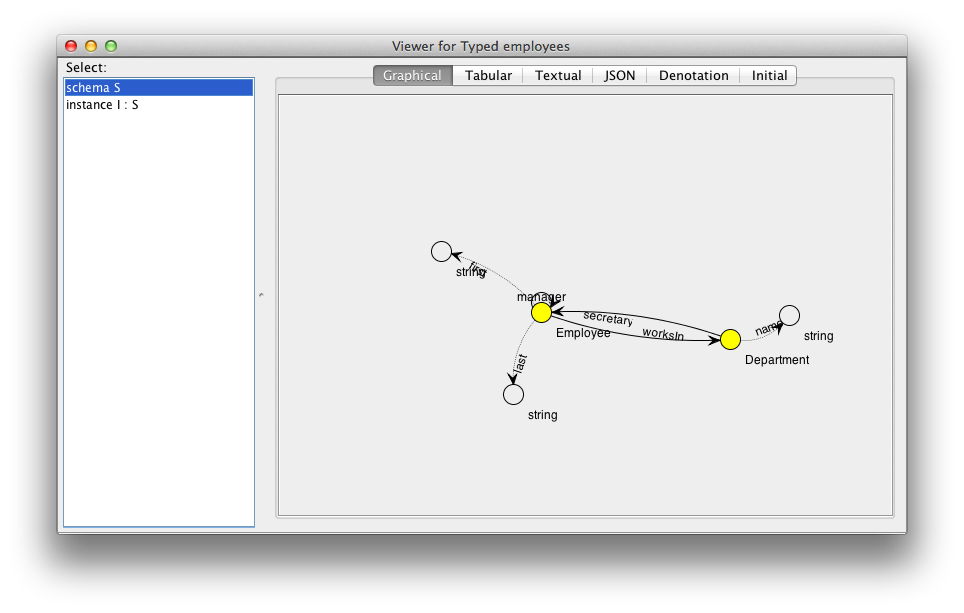
\includegraphics[width=6in]{schema}
\end{center}

Note that the four sections, ``nodes'', ``attributes'', ``arrows'', and ``equations'' are ended with semi-colons, and must appear in that order, even when a section is empty.  The ``denotation'' prints the category that the schema denotes.

\subsubsection{Cyclic Schemas}

By default, FQL requires all schemas to be finite.  Such schemas can be cyclic, provided they have ``finitizing'' equations -- see the ``Typed Employees'' example.   However, FQL can implement $\Delta,\Sigma$ migrations over infinite schemas, provided the ``do not validate mappings'' option is checked.  When checked, mappings will not be checked for functorality, and inputting a non-functorial mapping may result in in undefined behavior.  

\subsubsection{Enumerations (User defined types)}
FQL supports named enumerations.  In the ``Enums'' example, we see:
\begin{verbatim}
enum color = { red, green, blue }
schema S = { nodes S_node;
	attributes S_att : S_node -> color; arrows; equations; }
\end{verbatim}

\subsubsection{Schema Mappings}
Next, load the ``typed delta'' example.  It defines two schemas, $C$ and $D$, and a mapping $F$ from $C$ to $D$:

 \begin{minipage}{0.4\textwidth}
\begin{verbatim} 


 schema C = {
 nodes T1, T2;
 attributes
   t1_ssn    : T1 -> string, 
   t1_first  : T1 -> string, 
   t1_last   : T1 -> string,
   t2_first  : T2 -> string, 
   t2_last   : T2 -> string, 
   t2_salary : T2 -> int;
 arrows; equations; 
}
    \end{verbatim}
  \end{minipage}
%  \quad
   \hspace{.5in} $\to_F$ \hspace{.5in}
  \begin{minipage}{0.4\textwidth}
\begin{verbatim} 
schema D = {
 nodes T;
 attributes
  ssn0    : T -> string, 
  first0  : T -> string,
  last0   : T -> string,
  salary0 : T -> int;
 arrows; equations;
}    
\end{verbatim} \end{minipage}
  
\begin{verbatim}
mapping F  = {
 nodes T1 -> T, T2 -> T;
 attributes
  t1_ssn -> ssn0,  t1_first  -> first0,  t1_last -> last0,
  t2_last -> last0,  t2_salary -> salary0,  t2_first -> first0;
 arrows;
} : C -> D
\end{verbatim}
A mapping $F : C \to D$ consists of three parts:
\begin{itemize}
\item a mapping from the nodes in $C$ to the nodes in $D$
\item a mapping from the attributes in $C$ to the attributes in $D$
\item a mapping from the arrows in $C$ to paths in $D$
\end{itemize}
A mapping must respect the equations of $C$ and $D$: if $p_1$ and $p_2$ are equal paths in $C$, then $F(p_1)$ and $F(p_2)$ must be equal paths in $D$.  If this condition is not met, FQL will throw an exception.  Our example mapping is rendered in the viewer as follows:

\begin{center}
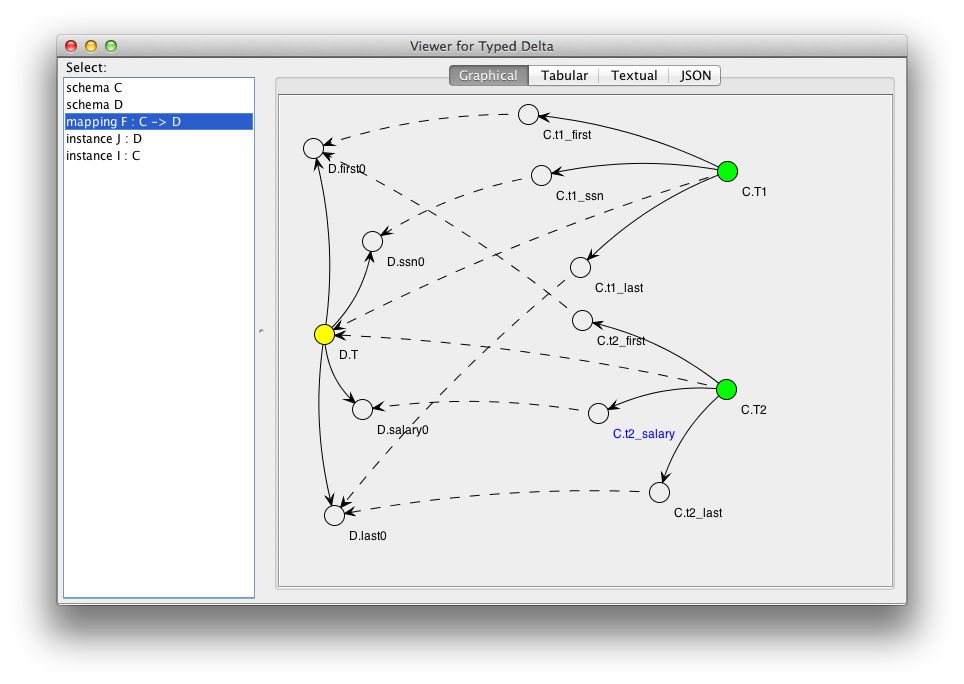
\includegraphics[width=4in]{mapping}
\end{center}

An identity mapping can be formed using the keyword ``id'' as follows:
\begin{verbatim}
mapping F = id C
\end{verbatim}
Mappings can be composed using the keyword ``then'' (parenthesis required) as follows:
\begin{verbatim}
mapping F = (G then H)
\end{verbatim}

\subsubsection{Union Schemas and Inclusion Mappings}
For convenience, FQL provides a ``macro'' to union two schemas together (which can fail, for example, when the two schemas have attributes with the same name but different types), and a ``macro'' for constructing inclusion mappings.  Details are in the ``Sub Schema'' example: 
\begin{verbatim}
schema ab = {
	nodes a, b; attributes atta : a -> string, attb : b -> string;
	arrows f : a -> b; equations; }

schema c = {nodes c; attributes attc : c -> string; arrows; equations;}

schema abc = (ab union c)
mapping F = subschema ab abc
\end{verbatim}

\subsubsection{Schema Flow}

In the viewer, select ``Schema Flow'' at the bottom left to see a graph where every vertex is a named schema, and every edge is a named mapping.  Clicking on a vertex or an edge will cause the viewer display to change to that schema or mapping.



\subsection{Instances}

Continuing with the built-in ``typed employees'' example, we see that it also contains FQL code that defines an instance of the schema $S$ defined in the previous section:

\begin{verbatim}
instance I = {
 nodes
  Employee -> { 101, 102, 103 },
  Department -> { q10, x02 };
  
 attributes
  first -> { (101, Alan), (102, Camille), (103, Andrey) },
  last  -> { (101, Turing), (102, Jordan), (103, Markov) },
  name  -> { (q10, AppliedMath), (x02, PureMath) };
  
 arrows
  manager -> { (101, 103), (102, 102), (103, 103) },
  worksIn -> { (101, q10), (102, x02), (103, q10) },
  secretary -> { (q10, 101), (x02, 102) };
} : S
\end{verbatim}

This declaration defines an instance $I$ that conforms to schema $S$.  This means that
\begin{itemize}
\item To each node/entity type corresponds a set of globally unique IDs.  In this example, the employee IDs are 101, 102, and 103, and the departmental IDs are q10 and x02.
\item Each attribute corresponds to a function that maps IDs to atoms.  In this example, we see that employee 101 is Alan Turing, employee 102 is Camille Jordan, employee 103 is Andrey Markov,  department q10 is AppliedMath, and department x02 is PureMath.
\item Each arrow $f : X \to Y$ corresponds to a function that maps IDs of entity type $X$ to IDs of entity type $Y$.  In this example, we see that Alan Turing and Andrey Markov work in the AppliedMath department, but Camille Jordan works in the PureMath department.
\end{itemize}

FQL assumes that every node, attribute, and arrow is stored as a binary table; node tables are stored as reflexive tables with types of the form $(x,x)$.  {\bf In addition, FQL assumes that the exact value of IDs are irrelevant, and in fact FQL will replace our IDs ``q10, x02, 101, 102'' and ``103''  with generated IDs 1,2,3,4,5.  Indeed, replacement of IDs will happen often with FQL data migration operations.} To visualize this instance, press ``compile'', select the instance from the viewer list, and click the ``tabular'' tab:

\begin{center}
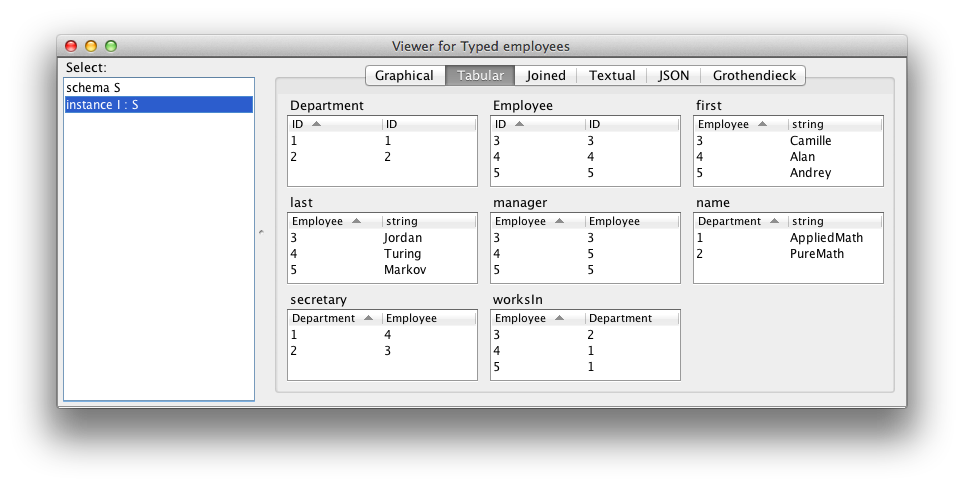
\includegraphics[width=5.5in]{instance}
\end{center}

To enter a string that contains spaces, simply quote it.  The ASWRITTEN keyword can automatically generate attributes based on node IDs (see ``Written macro'' example).

\subsubsection{Category of Elements}

Provided the ``Elements'' option is enabled, the ``Elements'' tab in an instance displays the instance as a category, ``the category of its elements''.  In this view, nodes are entities and arrows are foreign-key correspondences. Th Elements view is well illustrated using the ``People'' example:

\begin{center}
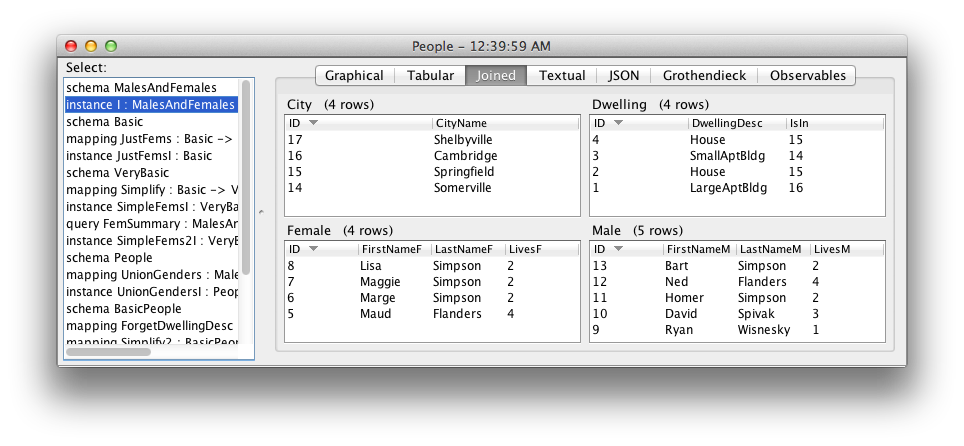
\includegraphics[width=4in]{people}
\end{center}

\begin{center}
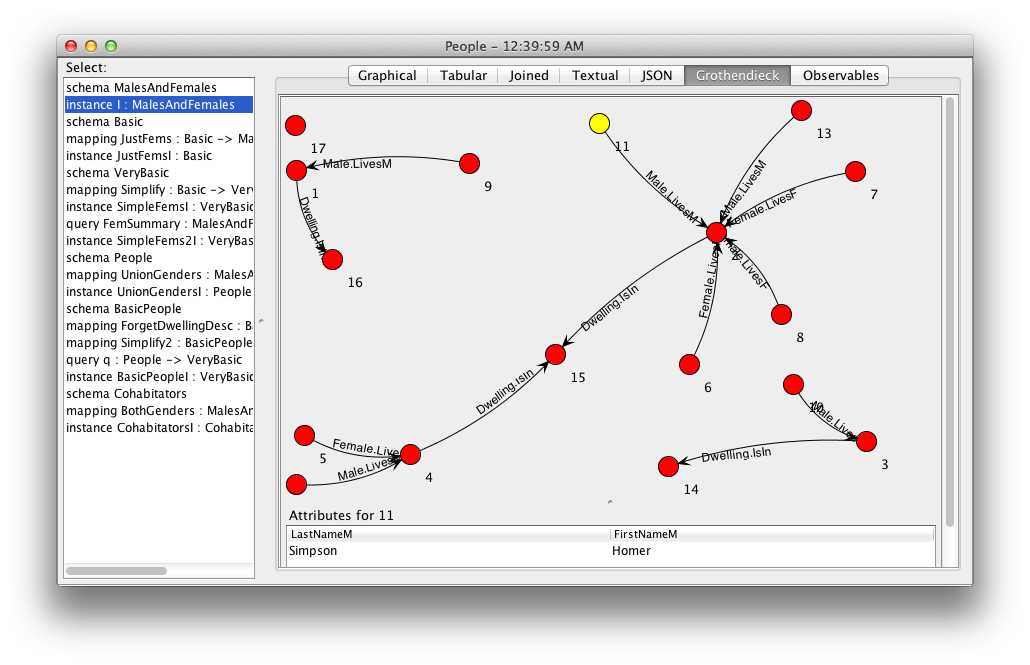
\includegraphics[width=6in]{elements}
\end{center}

\subsubsection{Relationalization and Observation}

Associated with each type of entity in an instance is an ``observation table''.  For an entity type/node $N$, the observation table joins together all attributes reachable by all paths out of $N$.  Consider the ``relationalize'' example:
\begin{verbatim}
schema C={
 nodes A;
  attributes a:A->string;
  arrows f:A->A;
  equations A.f.f.f.f=A.f.f; }

instance I:C={
	nodes A->{1,2,3,4,5,6,7};
	attributes a->{(1,1),(2,2),(3,3),(4,1),(5,5),(6,3),(7,5)};
	arrows f->{(1,2),(2,3),(3,5),(4,2),(5,3),(6,7),(7,6)}; }

instance RelI:C=relationalize I
transform trans = RelI.relationalize
\end{verbatim}

\begin{center}
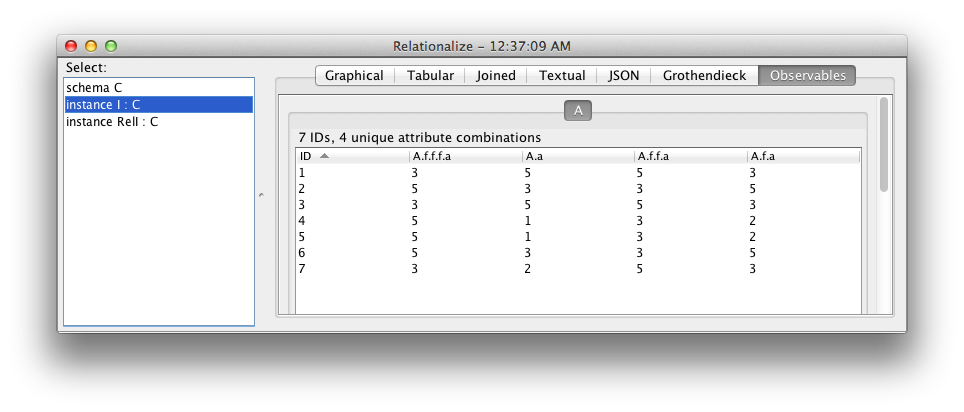
\includegraphics[width=6in]{observe}
\end{center}

The operation ``relationalize'' will equate IDs that are not distinguished by attributes.  In this example, 7 rows would collapse to 4. The transform {\tt RelI.relationalize} gives the mapping of the 7 rows to the 4 rows. The relationalize operation is expensive, but necessary to faithfully implement relational projection on relations that have been encoded as functorial instances.  The observation view displays the relationalization of every instance and can be enabled in the options menu.  The Observables pane is never computed via JDBC.

\begin{itemize}
\item {\bf If your program is taking too long to run, try disabling the observables and elements GUI panes.}  FQL computes all GUI panes; they are not computed lazily. 
\end{itemize}

\subsubsection{Transformations (database homomorphisms)}

For each schema $T$ and $T$-instances $I$,$J$, a {\it transformation} $f : I \to J$ is a database homomorphism from $I$ to $J$: for each node $n \in T$, $f_n$ is a constraint and attribute respecting function from $I_n$ IDs to $J_n$ IDs.  Transformations are illustrated in the ``Transform2'' example:
\begin{verbatim}
schema C = {
	nodes A;
	attributes att:A->string;
	arrows f:A->A;
	equations A.f.f.f=A.f.f;
}

instance I = {
	nodes A->{1,2,3,4,5};
	attributes att->{(1,common),(2,common),(3,common),(4,common),(5,common)};
	arrows f->{(1,2),(2,3),(3,3),(4,2),(5,3)};
} : C 

instance J = {
	nodes A->{1,2,3};
	attributes att->{(1,common),(2,common),(3,common)};
	arrows f->{(1,2),(2,3),(3,3)};
} : C 

//transform BadTransform = {
//	nodes A->{(1,1),(2,2),(3,4)};
//} :  J -> I

transform GoodTransform1 = {
	nodes A->{(1,1),(2,2),(3,3)};
} :  J -> I

transform GoodTransform2 = {
	nodes A->{(1,1),(2,2),(3,3),(4,1),(5,2)};
} :  I -> J
\end{verbatim}

The viewer for transforms is similar to the ``Elements'' viewer instances, except that IDs are colored according to their corresponding nodes.

\subsubsection{Instance Flow}
In the viewer, select ``Instance Flow'' at the bottom left to see a graph where every vertex is a named instance, and every edge is a data migration operation.  Clicking on a vertex or an edge will cause the viewer display to change to that instance or data migration.  Note that some data migration operations may not be explicitly named; in this case, the operation will still display, but the operation cannot be selected by the list of named FQL declarations.


\subsubsection{Visual Editing}

Instances (and Transforms) can be editing using a graphical, tabular interface similar to how instances are rendered.  To visually edit an instance (transform), right-click on an instance (transform) in the main text editor and select ``visually edit''.  A modal dialog will pop up; by clicking on a node, the joined view of that node appears.  Double-clicking in a cell allows to change the contents of the cell; enter finalizes the change.  Rows can be selected using the shift key.  Note that instances (transforms) need not be well-formed to be edited, although the FQL program must parse and the schema of the instance must be well-formed.  Instances (transforms) can be edited in such a way that they output non well-formed FQL.  Empty values in cells are treated as empty strings.  

\subsection{Data Migration}

Associated with a mapping $F : C \to D$ are three data migration operators:
\begin{itemize}
\item $\Delta_F$, taking $D$ instances to $C$ instances, roughly corresponding to projection
\item $\Pi_F$, taking $C$ instances to $D$ instances, roughly corresponding to join
\item $\Sigma_F$, taking $C$ instances to $D$ instances, roughly corresponding to union
\end{itemize}

In general, certain restrictions must be placed on $F$ to guarantee the above operations exist. We now describe each in turn.  

\subsubsection{Delta}

Continuing with the ``typed delta'' example, we see that the FQL program also defines a $D$-instance $J$, and computes $I := \Delta_F(J)$:

\begin{verbatim}
instance I = delta F J
\end{verbatim}

Graphically, we have

\begin{center}
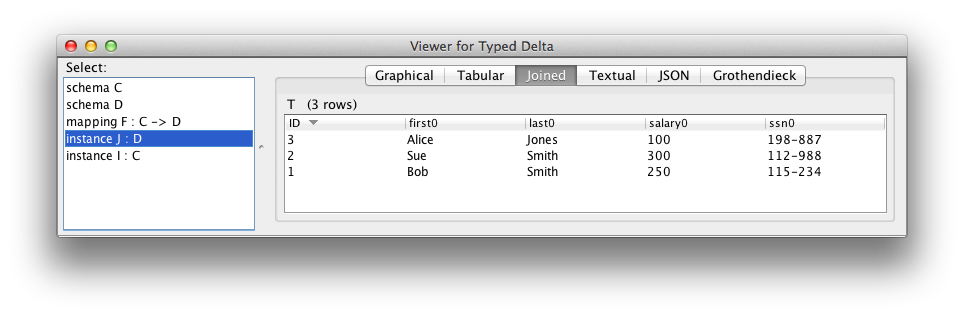
\includegraphics[width=6in]{deltaJ}

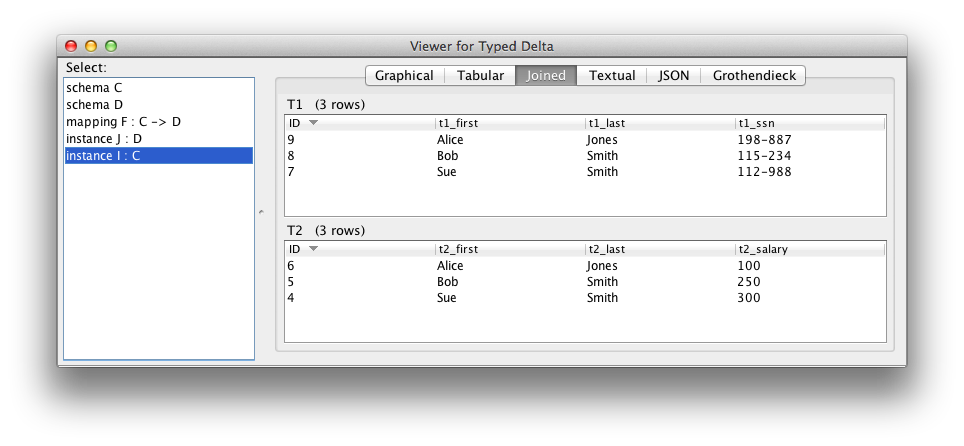
\includegraphics[width=6in]{deltaI}
\end{center}

In effect, we have projected the columns salary0 and last0 from $J$.  

\subsubsection{Pi}

Load the ``typed pi'' example:

 \begin{minipage}{0.4\textwidth}
\begin{verbatim} 


 schema C = {
 nodes 
 	c1, 
 	c2;
 attributes
	att1 : c1 -> string,
	att2 : c1 -> string, 
	att3 : c2->string;
 arrows;
 equations;
}
    \end{verbatim}
  \end{minipage}
%  \quad
   \hspace{.5in} $\to_F$ \hspace{.5in}
  \begin{minipage}{0.4\textwidth}
\begin{verbatim} 
schema D = {
 nodes 
 	d;
 attributes
 	a1 : d -> string, 
 	a2 : d -> string, 
 	a3 : d -> string;
 arrows;
 equations;
}  
\end{verbatim} \end{minipage}
\begin{verbatim}
mapping F = {
 nodes c1 -> d, c2 -> d;
 attributes att1 -> a1,  att2 -> a2, att3 -> a3;
 arrows;
}  : C -> D
\end{verbatim}
This example defines an instance $I : C$ and computes $J := \Pi_F(I)$:
\begin{verbatim}
instance J = pi F I
\end{verbatim}
Graphically, this is rendered as:

\begin{center}
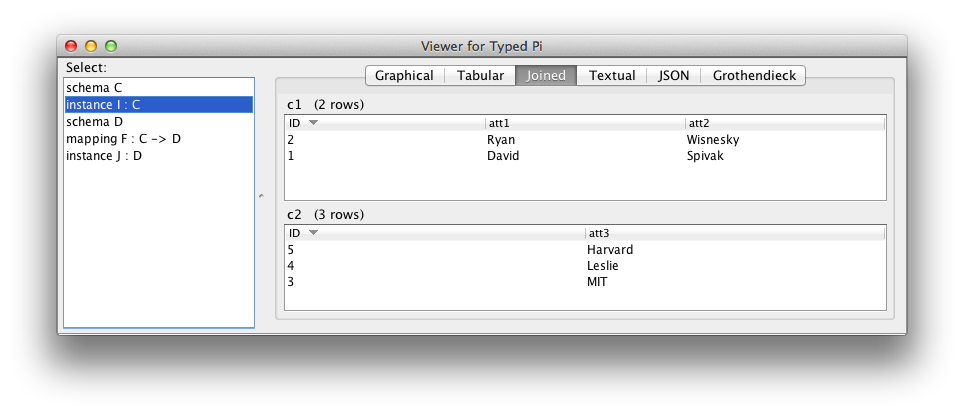
\includegraphics[width=5in]{piI}

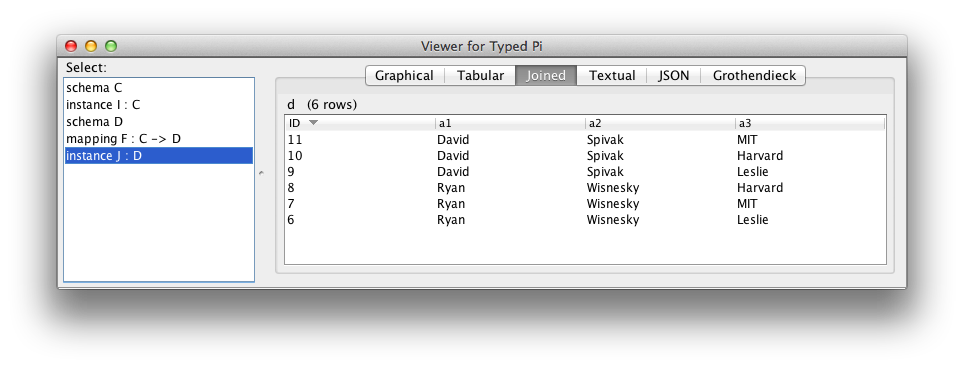
\includegraphics[width=5in]{piJ}
\end{center}

We see that we have computed the cartesian product of tables $c_1$ and $c_2$.  Note that the attribute mapping part of $F$ must be a bijection for $\Pi_F$ to be defined; if this condition fails FQL will throw an exception.  There is menu option to allow surjections to be used instead of bijections; we are confident that surjections behave correctly, but haven't proven all requisite theorems.

\subsubsection{Sigma}


Load the ``sigma'' example:

 \begin{minipage}{0.4\textwidth}
\begin{verbatim} 


schema C = {
 nodes
 	a1, a2, a3, b1, b2, c1, c2, c3, c4;
 	
 attributes;
 
 arrows
  g1 : a1 -> b1, 
  g2 : a2 -> b2, 
  g3 : a3 -> b2,
  h1 : a1 -> c1, 
  h2 : a2 -> c2, 
  h3 : a3 -> c4;
 	
 equations;
}    \end{verbatim}
  \end{minipage}
%  \quad
   \hspace{.5in} $\to_F$ \hspace{.5in}
  \begin{minipage}{0.4\textwidth}
\begin{verbatim} 
schema D = {
 nodes A, B, C;
 	
 attributes;
 
 arrows
  G : A -> B, 
  H : A -> C;
	
 equations;
}
\end{verbatim} \end{minipage}
\begin{verbatim}
mapping F = {
 nodes 
  a1 -> A, a2 -> A, a3 -> A,
  b1 -> B, b2 -> B, 
  c1 -> C, c2 -> C, c3 -> C, c4 -> C;
  	
 attributes;
 
 arrows 
  g1 -> A.G, g2 -> A.G, g3 -> A.G,
  h1 -> A.H, h2 -> A.H, h3 -> A.H;
} : C -> D
\end{verbatim}
This example defines an instance $I : C$ and computes $J := \Sigma_F(I)$:
\begin{verbatim}
instance J : D = sigma F I
\end{verbatim}
Graphically, this is rendered as:

\begin{center}
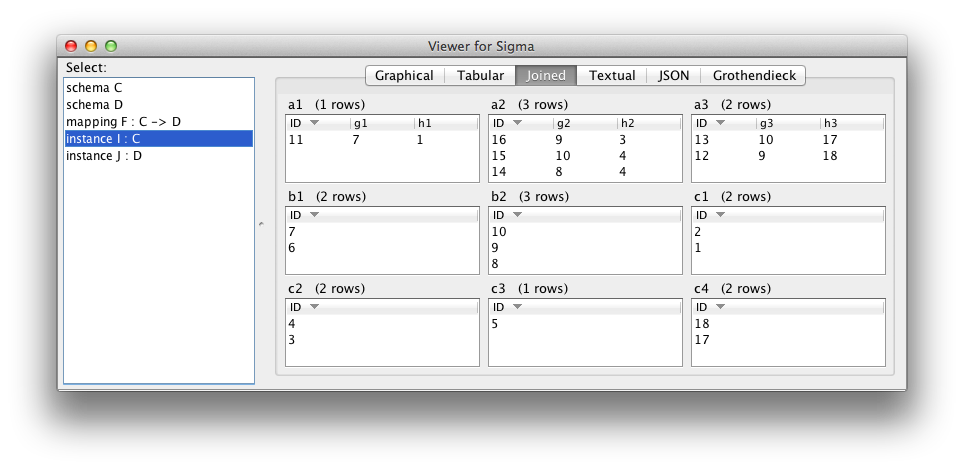
\includegraphics[width=4in]{sigmaI}

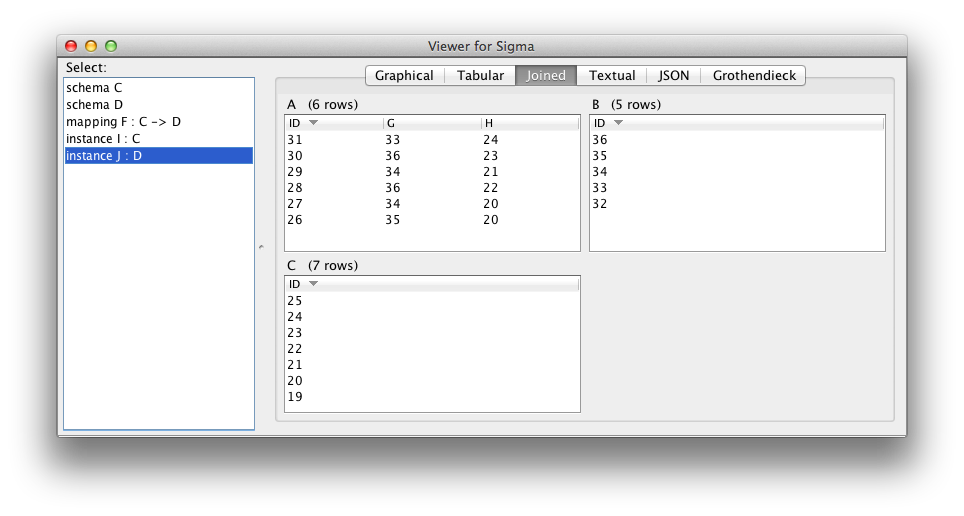
\includegraphics[width=5in]{sigmaJ}
\end{center}

We see that we have computed union of tables $a_1$, $a_2$, and $a_3$ as $A$ (6 rows), the union of tables $b_1, b_2$ as $B$ (5 rows), and the union of $c_1, c_2, c_3$ and $c_4$ as $C$ (7 rows). 

\subsubsection{Unrestricted Sigma}

For $\Sigma_F$ to implementable in SQL, the functor $F$ must satisfy the special condition of being a {\it discrete op-fibration}, which basically means ``union compatible in the sense of Codd''.  Mathematically, it is possible to define $\Sigma$ for any schema mapping, not just mappings that are union-compatible.  Such an unrestricted sigma is known as a ``Left-hand'' extension.  The FQL IDE can compute such ``unrestricted'' sigmas, indicated by the keyword ``SIGMA'' (all caps).  See the ``full sigma'' example for details.  

Note that typed (i.e., containing attributes) full sigmas 1) can create null values if that option is checked (but this feature is experimental and dangerous), and 2) can fail if it would require equating two distinct constants such as ``alice'' and ''bob''.  Full sigma can be implemented using EDs, and indeed, we have proved that every chase sequence of these EDs corresponds to a run of the full sigma algorithm.  


\subsubsection{Data Migration on Transformations}

If $f : I \to J$ is a transformation, then so is $\Delta_F(f) : \Delta_F(J) \to \Delta_F(I)$, $\Sigma_F(f) : \Sigma_F(I) \to \Sigma_F(J)$, $\Pi_F(f) : \Pi_F(f) : \Pi_F(I) \to \Pi_F(J)$, and $relationalize(f) : relationalize(I) \to relationalize(J)$.   See the All Syntax example for details.

\begin{itemize}
\item Note: For a full $\Sigma$ the input transform must be explicitly named.  While not required in theory, this restriction is necessary to allow full sigma on transforms to easily work with external SQL engines that cannot natively support full sigmas.
\end{itemize}

\subsubsection{Monads and Comonads}

For every $F$ and $I$, there are canonical transforms $return : I \to \Delta_F(\Sigma_F(I))$ and $coreturn : \Sigma_F(\Delta_F(I)) \to I$, as well as canonical transforms $return : I \to \Pi_F(\Delta_F(I))$ and $coreturn : \Delta_F(\Pi_F(I)) \to I$.  These transforms come from the mathematical theory of {\it monads}.  They are illustrated in the Sigma and Pi examples, but here we will focus on the ``Connected Components'' example. To load it, you must enable ``all examples'' in the options menu.  The basic idea is that these transforms provide a connection between $I$ and $\Sigma_F(I)$, and between $\Pi_F(I)$ and $I$.

\begin{verbatim}
schema Graph = {
	nodes arrow,vertex;
	attributes;
	arrows src:arrow->vertex,tgt:arrow->vertex;
	equations;
}

//has 4 connected components
instance G = {
	nodes arrow->{a,b,c,d,e}, vertex->{t,u,v,w,x,y,z};
	attributes;
	arrows
		src->{(a,t),(b,t),(c,x),(d,y),(e,z)},
		tgt->{(a,u),(b,v),(c,x),(d,z),(e,y)};
} : Graph

schema Terminal = {
	nodes X;
	attributes;
	arrows;
	equations;
} 

mapping F = {
	nodes arrow->X, vertex->X;
	attributes;
	arrows src->X, tgt->X;
} : Graph -> Terminal

//has 4 rows
instance Components=SIGMA F G

//puts 4 rows into vertex, 4 rows into arrow, corresponding to the connected components
instance I = delta F Components

//gives the transform from the original graph to the connected components
transform t = I.return
\end{verbatim}

In this example, instances on schema $Graph$ are representations of (directed) (multi) graphs: instance $G$ contains 7 vertices and 5 edges.  Running the example, we see that $Components$ has 4 elements:
\begin{verbatim}
//instance G
{
nodes
arrow -> { 1, 2, 3, 4, 5 },
vertex -> { 6, 7, 8, 9, 11, 10, 12 }
 ;
attributes

 ;
arrows
tgt -> { (3,10), (2,11), (5,8), (1,7), (4,6) },
src -> { (3,12), (2,12), (4,8), (5,6), (1,7) };
}

//instance Components
{
nodes X -> { 15, 14, 20, 12 };
attributes;
arrows;
}
\end{verbatim}
We might wish to know which connected component each arrow and vertex is a part of.  Since the connected components were computed by $\Sigma$, we can use $\Delta$ to compute another graph whose arrows are vertices are the connected components.  Then, the return monad operation provides a transform from the original graph to this new graph. 
\begin{verbatim}
//instance I
{
nodes
arrow -> { 32, 31, 30, 29 },
vertex -> { 33, 34, 35, 36 }
 ;
attributes

 ;
arrows
tgt -> { (31,35), (30,34), (32,36), (29,33) },
src -> { (31,35), (30,34), (32,36), (29,33) };
}

//transform t : G -> I
{nodes
arrow -> {(4,32),(5,32),(3,31),(1,30),(2,31)},
vertex -> {(11,35),(10,35),(12,35),(8,36),(7,34),(6,36),(9,33)};
}
\end{verbatim}
We can see above that $t$ associates certain arrows, such as $2$ and $3$ to the same connected component ($31$).

\subsection{Queries}
In SQL, unions of select-from-where clauses are the common programming idiom.  In FQL, the common idiom is $\Sigma$s of $\Pi$s of $\Delta$s.  Load the ``composition'' example:

\begin{verbatim}
schema S = { nodes s ; attributes; arrows; equations; }
schema T = { nodes t ; attributes; arrows; equations; }
schema B = { nodes b1,b2; attributes; arrows; equations; }
schema A = { nodes a1,a2,a3; attributes; arrows; equations; }

mapping s  = { nodes b1 -> s, b2 -> s; attributes; arrows; }: B -> S
mapping f = { nodes b1 -> a1, b2 -> a2 ; attributes; arrows; } : B -> A
mapping t  = { nodes a1 -> t, a2 -> t, a3 -> t ; attributes; arrows; }: A -> T

query q1  = delta s pi f sigma t
\end{verbatim}

In general, a query is simply a convenient shorthand.

\begin{center}
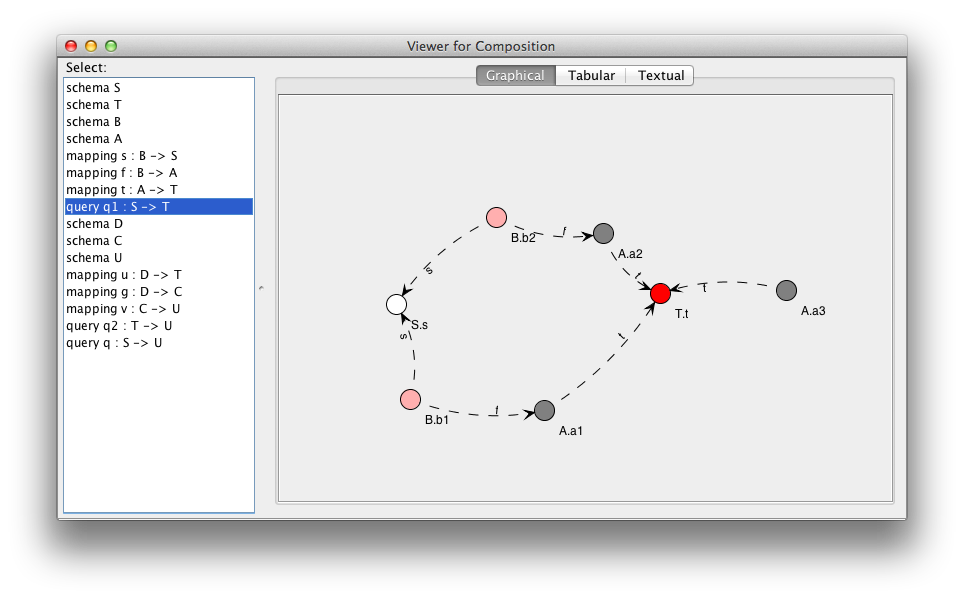
\includegraphics[width=6in]{composition}
\end{center}
 Queries may be evaluated using the keyword ``eval'':
\begin{verbatim}
instance J  = ...
instance I  = eval q1 J
\end{verbatim}

\subsubsection{Composition}
FQL includes special support for composing queries.  Continuing with the ``composition'' example, we see that it defines another query:

\begin{verbatim}
schema D = { nodes d1,d2 ;  attributes; arrows; equations; }
schema C = { nodes c ;  attributes; arrows; equations; }
schema U = { nodes u ;  attributes; arrows; equations;}

mapping u  = { nodes d1 -> t, d2 -> t ;  attributes; arrows;}: D -> T
mapping g = { nodes d1 -> c, d2 -> c ;  attributes; arrows;}: D -> C 
mapping v  = { nodes c -> u ;  attributes; arrows; }: C -> U

query q2 = delta u pi g sigma v
\end{verbatim}
We compose our two queries as follows (parenthesis required):
\begin{verbatim}
query q  = (q1 then q2)
\end{verbatim}
FQL supports another top-level type, the {\tt QUERY}, for free compositions of data migration functors (i.e., not triplets).  Full sigma ({\tt SIGMA}) can be used with {\tt QUERY}.

\subsubsection{Generating Queries from Schema Correspondences}

FQL has experimental support for generating queries from attribute correspondences (schema matching).  Because such mappings are often not discrete op-fibrations, FQL defines these using {\tt QUERY}.  Many different queries can be generated from a correspondence; these are identified by strings.  Queries can be evaluated on instances with {\tt EVAL}, similarly to {\tt eval}.  Load the ``Schema Matching'' example (requires the additional examples options):
\begin{verbatim}
schema ab = { nodes a, b;
	attributes atta : a -> string, attb : b -> string; arrows f : a -> b;
	equations; }

schema c = { nodes c; attributes attc : c -> string; arrows ; equations; }

QUERY q1 = match {(atta,attc),(attb,attc)} ab c "delta sigma forward"
QUERY q2 = match {(atta,attc),(attb,attc)} ab c "delta sigma backward"
QUERY q3 = match {(atta,attc),(attb,attc)} ab c "delta pi forward"
QUERY q4 = match {(atta,attc),(attb,attc)} ab c "delta pi backward"
\end{verbatim}
The viewer displays the associated data migration queries:
\begin{verbatim}
(SIGMA {nodes c -> right_c; attributes attc -> right_attc; 
arrows;} : c -> 
 {nodes left_a, left_b, right_c;
  attributes  left_atta : left_a -> string, left_attb : left_b -> string,
   right_attc : right_c -> string;
arrows left_f : left_a -> left_b; equations; } 
then 
delta {nodes b -> left_b, a -> left_a;
attributes attb -> left_attb, atta -> left_atta;
arrows f -> left_a.left_f;
} : ab ->  { nodes left_a, left_b, right_c;
attributes
left_atta : left_a -> string, left_attb : left_b -> string, 
right_attc : right_c -> string;
arrows left_f : left_a -> left_b; equations; })
\end{verbatim}



%\newpage

\section{Programming with FQL}

\subsection{Categorical Combinators}

FQL contains programming capabilities to FQL in the guise of {\it categorical combinators}.  Intuitively, these combinators are a standard functional programming language similar to e.g., point-free Haskell. Their semantics derives from the fact that the category of schemas and mappings is bi-cartesian closed, and for each $T$, the category of $T$-instances and their homomorphisms is a topos.  Hence, schemas and mapping can be programmed using the variable-free form of the simply-typed $\lambda$-calculus, and instances and transforms can be programmed using the variable-free form of higher-order logic.   The main GUI contains a type-checker menu option.

\subsection{Programming with Schemas and Mappings}
Schema and mapping expressions can be freely nested:
\begin{verbatim}
enum color = {red, green, blue}

schema C = {nodes; attributes; arrows; equations;}
schema C1 = void
schema C2 = unit {string, int, color}
schema C3 = (C + C)
schema C4 = (C * C)
schema C5 = (C union C)
schema C6 = opposite C
schema C7 = (C ^ C)

mapping F = id C
mapping F1 = (F then F)
mapping F2 = {nodes; attributes; arrows;} : C -> C
mapping F3 = inl C C
mapping F4 = inr C C
mapping F5 = (F3 + F4)
mapping F6 = fst C C
mapping F7 = snd C C
mapping F8 = (F6 * F7)
mapping F9 = void C
mapping F10= unit {string, int, color} C
mapping F13 = subschema C C5
mapping F14 = opposite F
mapping F11= eval C C
mapping F12= curry id (C*C)
mapping F15= iso1 C C
mapping F16= iso2 C C
\end{verbatim}
Given a signature $C$, $opposite \ C$ defines the signature with all the arrows reversed, and given a mapping $F : C \to D$, $opposite \ F : opposite \ C \to opposite \ D$.

\subsubsection{Co-products of Schemas}

The ``Co-products Schema'' example illustrates co-products of schemas:

\begin{verbatim}
schema C = { nodes a, b; attributes att : a -> string; 
arrows f : a -> b, g : a -> a; equations a.g = a; }

schema D = { nodes a; attributes att : a -> string; arrows ; equations ; }

schema E = (C + D)
mapping f = inl C D
mapping g = inr C D
mapping h = (f + g) // this is actually the identity!

schema X = void
mapping q = void C

schema Y = ((C + (C + C)) + void)
\end{verbatim}

Schemas $C$ and $D$ are disjointly unioned in $E := C + D$: each node in $C$ appears in $C+D$ (albeit with an automatically generated name), and each node in $D$ appears in $C+D$.  Similarly, the attributes and arrows of $C$ and $D$ are injected into $C+D$.  The injection mappings have types $inl \ C \ D : C \to C+D$ and $inr \ C \ D : D \to C+D$.  Given mappings $f : C \to X$ and $g : D \to X$, mapping $(f + g)$ (parenthesis required) has type $C+D \to X$.  Co-products obey the equations
$$
inl ; (f + g) = f \ \ \ \ inr ; (f + g) = g \ \ \ \ (inl + inr) = id
$$
All manipulations of co-product schemas must be done using $inl$, $inr$, and $(+)$.  The empty schema is written $void$ and for every schema $C$, the mapping $void \ C : void \to C$ is the unique (empty) map to $C$.  The empty schema is a unit for co-products in the sense that $C$ and $void + C$ are isomorphic.

\subsubsection{Products of Schemas}
The ``Products' Schema' example illustrates products of schemas:
\begin{verbatim}
schema S = {
	nodes a, b, c;
	attributes att:a->string;
	arrows f:a->b, g:b->c, h:a->c;
	equations a.h = a.f.g;
}

schema T = {
	nodes x, y;
	attributes att:x->string;
	arrows u:x->y, z:x->y;
	equations x.u = x.z;
}

mapping F = {
	nodes x -> a, y -> c;
	attributes att->att;
	arrows u -> a.f.g, z->a.f.g;
} : T -> S 

schema A = (S * T)
mapping p1 = fst S T
mapping p2 = snd S T
mapping p = (p1*p2) //is identity

schema X = unit {string}
mapping H = unit {string} T
\end{verbatim}
 Schemas $C$ and $D$ are multiplied in $E := C \times D$: nodes in $C \times D$ are pairs $(c,d)$ where $c \in C$ and $d \in D$, albeit with automatically generated names.  Hence, the attributes and arrows of $C\times D$ are pairs of attributes and arrows from $C$ and $D$.  The projection mappings have types $fst \ C \ D : C \times D \to C$ and $snd \ C \ D : C \times D \to D$.  Given mappings $f : X \to C$ and $g : X \to D$, mapping $(f \times g)$ (parenthesis required) has type $X \to C\times D$.  Products obey the equations
$$
(f \times g) ; fst = f \ \ \ \ (f \times g) ; snd = g \ \ \ \ (fst \times snd) = id
$$
All manipulations of product schemas must be done using $fst$, $snd$, and $(\times)$.  The schema with one node and one attribute for each type $\{ t_1, \ldots \}$ is written $unit \ \{ t_1, \ldots \}$ and for every schema $C$, the mapping $unit \ \{t_1, \ldots \} \ C : C \to unit \{ t_1, \ldots\}$ is the unique (collapsing) map to $unit \ \{t_1, \ldots\}$.  The terminal schema is a unit for products in the sense that $C$ and $unit \ \{t_1, \ldots \} \times C$ are isomorphic.

\subsubsection{Exponentials of Schemas}
The ``Exponentials'' example illustrates exponentials of schemas:
\begin{verbatim}
schema A = {
	nodes a1, a2;
	attributes;
	arrows af : a1 -> a2;
	equations;
}

schema B = {
	nodes b1, b2, b3;
	attributes;
	arrows bf1 : b1 -> b2, bf2 : b2 -> b3;
	equations;
}

schema S = (A^B)

mapping eta = curry eval A B // (= id)

mapping F = unit {} (A*B) //can use any F for beta, we choose this one

mapping beta = (  ((fst A B then curry F) * (snd A B then id B)) 
                                then eval unit {} B  ) // (= F)
\end{verbatim}
The nodes of $(C^D)$ (parenthesis required) are mappings $D \to C$ and the arrows of $C^D$ are natural transformations between mappings, albeit with automatically generated names.  There are no attributes in $C^D$.  There is an ``evaluation'' mapping $eval \ C \ D : C^D \times D \to C$, and given a mapping $f : A \times B \to C$ such that $A$ has no attributes, there is a ``currying'' mapping $curry \ f : A \to C^B$.  Exponentials obey equations
$$
curry \ eval = id \ \ \ \ \ (proj_1 ; f \times proj_2 ; id) ; eval = f
$$
All manipulations of exponential schemas must be done using $eval$, $curry$, and $(-^-)$.  

\subsubsection{Isomorphisms of Schemas}
 If $S$ and $T$ are isomorphic schemas, then $iso_1 : S \to T$ and $iso_2 : T \to S$ will be one such isomorphism, satisfying $iso_1 ; iso_2 = id$ and $iso_2 ; iso_1 = id$.  Isomorphisms are particularly useful to convert between schemas with auto generated names and user defined names.  For example, suppose $A\times B$ has four nodes; because the schema is a product, the nodes will automatically be named $node1, node2, node3, node4$.  If $C$ is a manually input schema with nodes $name, age, date, location$, then $iso$ can be used to map between $A\times B$ and $C$.  See the ``Auto Iso'' example for details (requires the ``all examples'' option). 

\subsection{Programming with Instances and Transformations}

For each schema $T$ and $T$-instances $I$,$J$, a {\it transformation} $f : I \to J$ is a database homomorphism from $I$ to $J$: for each node $n \in T$, $f_n$ is a constraint and attribute respecting function from $I_n$ IDs to $J_n$ IDs.  Transformations are The following illustrates all FQL syntax for programming with instances and transformations:

\begin{verbatim}
query q = delta F pi F sigma F
query p = (q then q)
//see Schema Matching example for available strings
QUERY Q1 = delta F
QUERY Q2 = SIGMA F
QUERY Q3 = pi F
QUERY Q4 = match {} C C "delta sigma forward"
QUERY Q5 = (Q1 then Q2)

instance I   = { nodes; attributes; arrows; } : C
instance I1  = delta F I
instance I2  = pi F I
instance I3  = sigma F I
instance I4  = relationalize I
instance I5  = SIGMA F I
instance I8  = (I + I1)
instance I10 = (I ^ I)
instance I9  = (I10 * I)
instance I11 = unit C
instance I12 = void C
instance I13 = prop C
instance I6  = external C name
instance I7  = eval q I
instance I7x = EVAL Q1 I

transform t1 = id I
transform t2 = (t1 then t1)
transform t3 = {nodes;} : I -> I
transform t4 = I8.inl
transform t5 = I8.inr
transform t6 = I8.(t4+t5)
transform t7 = I9.fst
transform t9 = I9.snd
transform t10 = I9.(t7*t9)
transform t12 = I11.unit I
transform t13 = I12.void I
transform t15 = delta I1 I1 id I
transform t16 = sigma I3 I3 id I
transform t20 = SIGMA I5 I5 t1
transform t17 = pi I2 I2 id I
transform t18 = relationalize I4 I4 id I
transform t19 = I4.relationalize
transform t21 = external I6 I6 name
transform t22 = I9.eval
transform t23 = I10.curry t22
transform t24 = iso1 I I
transform t25 = iso2 I I
transform t26 = I13.true I11
transform t27 = I13.false I11
transform t28 = I13.char t26
instance Is = kernel t28
transform t29 = Is.kernel

////(co)monads also work for SIGMA and pi
instance I3X = delta F I3
transform I3Xa = I3X.return
instance I1X = sigma F I1
transform I1Xa = I1X.coreturn

drop I t1
\end{verbatim}
Note that equality for instances is nominal, meaning that instance names matter; if $I := E$ and $J := E$ are two instances, then $I \neq J$ even though $I$ and $J$ have the same definition.  Indeed, $I$ and $J$ will have different GUIDs. As a result the FQL language of instances and transformations is somewhat different than the FQL language of schemas and mappings.  Transforms may be freely nested, but Instances cannot be, as they rely on effectful SQL operations.

\subsubsection{Co-products of Instances}

The ``Co-products'' example illustrates co-products of instances (of the same schema):

\begin{verbatim}
schema S = {
	nodes a, b;
	attributes att : a -> string;
	arrows f : a -> b;
	equations;
}

instance I = {
nodes a -> {1,2}, b -> {3};
attributes att -> {(1,one),(2,two)};
arrows f -> {(1,3),(2,3)};
} : S

instance J = {
nodes a -> {a,b,c}, b -> {d,e};
attributes att -> {(a,foo),(b,bar),(c,baz)};
arrows f -> {(a,d),(b,e),(c,e)};
} : S

instance A = (I + J)
transform K = A.inl
transform L = A.inr
transform M = A.(K + L) //is id

instance N = void S
transform O = N.void J
\end{verbatim}
Instances $I$ and $J$ are unioned in $A := I + J$: each ID in $I$ appears in $A$ (albeit with a fresh, automatically generated name), and each ID in $J$ appears in $A$.  Similarly, the attributes and arrows of $I$ and $J$ are injected into $A$.  The injection transformations have types $A.inl \ I \to A$ and $A.inr \ J \to A$.  Given transformations $f : I \to X$ and $g : J \to X$, transformation $A.(f + g)$ (parenthesis required) has type $A \to X$.  The global unique ID assumption ensures all unions are disjoint. Co-products obey the equations
$$
A.inl ; A.(f + g) = f \ \ \ \ A.inr ; A.(f + g) = g \ \ \ \ A.(A.inl + A.inr) = id
$$
All manipulations of co-product instances must be done using $inl$, $inr$, and $(+)$.  The empty instance $U$ of schema $T$ is written $U := void \ T$ and for every instance $V$ of type $T$, the mapping $U.void \ V : U \to V$ is the unique (empty) map from $V$.  The empty instance is a unit for co-products in the sense that $V$ and $void + V$ are isomorphic.

\subsubsection{Products of Instances}

The ``Products'' example illustrates products of instances (of the same schema):

\begin{verbatim}
schema S = {
	nodes a, b;
	attributes att : a -> string;
	arrows f : a -> b;
	equations;}

instance I = {
nodes a -> {1,2}, b -> {3};
attributes att -> {(1,common),(2,common)};
arrows f -> {(1,3),(2,3)};
} : S

instance J = {
nodes a -> {a,b,c}, b -> {d,e};
attributes att -> {(a,common),(b,common),(c,baz)};
arrows f -> {(a,d),(b,e),(c,e)};
} : S

instance A = (I * J)
transform K = A.fst
transform L = A.snd
transform M = A.(K * L) //is id

schema X = {
	nodes a;
	attributes;
	arrows;
	equations;
}

instance N = unit X

transform O = N.unit N
\end{verbatim}
Instances $I$ and $J$ are joined in $A := I \times J$: each (fresh) ID in $I\times J $ corresponds to a pair of ids $(i,j)$ with $i \in I$ and $j \in J$ such that the attributes of $i$ and $j$ match. The attributes and arrows of $I$ and $J$ are multiplied into $I\times J$.  The projection transformations have types $A.fst \ A \to I$ and $A.snd \ A \to J$.  Given transformations $f : X \to I$ and $g : X \to J$, transformation $A.(f \times g)$ (parenthesis required) has type $X \to A$.  Products obey the equations
$$
 A.(f \times g) ; A.fst = f \ \ \ \ A.(f \times g) ; A.inr = g \ \ \ \ A.(A.fst \times A.snd) = id
$$
All manipulations of product instances must be done using $fst$, $snd$, and $(\times)$.  The terminal instance $U$ of schema $T$ (where $T$ has only enum (or no) attributes) is written $U := unit \ T$ and for every instance $V$ of type $T$, the mapping $U.unit \ V : V \to U$ is the unique (collapsing) map to $U$.  The unit instance is a unit for products in the sense that $V$ and $unit \times V$ are isomorphic.  See the ``Products'' example for details.
 
\subsubsection{Exponentials of Instances}

The ``Exponentials'' example illustrates exponentials of instances (on the same schema).  Note that exponentials cannot be implemented with SQL.
\begin{verbatim}
schema C = {
         nodes a, b;
         attributes;
         arrows f : a -> b;
         equations;
}

instance I = {
         nodes a -> {1,2,3}, b -> {4,5};
         attributes;
         arrows f -> {(1,4),(2,5),(3,5)};
} : C

instance J = {
         nodes a -> {1,2}, b -> {4};
         attributes;
         arrows f -> {(1,4),(2,4)};
} : C

instance K = (J^I)

instance M = (K*I) 

transform trans = M.eval

transform idx = K.curry trans //eta
\end{verbatim}
For each $c \in C$, the IDs of $(J^I)(c)$ correspond to transformations $H_c \times I \Rightarrow J$, where $H_c$ is the ``representable instance'' whose IDs at $H_c(d)$ correspond to paths $c \to d$.  There is an ``evaluation'' transform $eval \ C \ D : C^D \times D \to C$, and given a transform $f : A \times B \to C$, there is a ``currying'' transform $curry \ f : A \to C^B$.  As shown in the above example, exponentials obey the ``beta'' and ``eta'' equations:
$$
curry \ eval = id \ \ \ \ \ (proj_1 ; f \times proj_2 ; id) ; eval = f
$$
All manipulations of exponential instances must be done using $eval$, $curry$, and $(-^-)$.  Parenthesis are required.  Note that exponentials can't be used with non-enum attributes.

 \subsubsection{Proposition Instances and Truth-value Transformations}
 
 The ``Prop'' example illustrates propositional instances (on the same schema).  Note that propositions cannot be implemented with SQL.
 \begin{verbatim}
/* you must disable: 
 *  - observables, elements, rdf for instances
 *  - graph for transforms
 */

enum dname = {AppliedMath, PureMath}
enum fname = {Alan, Camille, Andrey}

schema S = { 
 nodes
 	Employee, Department;
 attributes
	name  : Department -> dname,
 	first : Employee -> fname;
 arrows
	manager   : Employee -> Employee,
	worksIn   : Employee -> Department,
	secretary : Department -> Employee;
 equations  
  	Employee.manager.worksIn = Employee.worksIn,
  	Department.secretary.worksIn = Department,
  	Employee.manager.manager = Employee.manager;
}

instance J = {
 nodes
	Employee -> { 101, 102, 103 },
	Department -> { q10, x02 };
 attributes
	first -> { (101, Alan), (102, Camille), (103, Andrey) },
	name  -> { (q10, AppliedMath), (x02, PureMath) };
 arrows
	manager -> { (101, 101), (102, 102), (103, 103) },
	worksIn -> { (101, q10), (102, x02), (103, q10) },
	secretary -> { (q10, 101), (x02, 102) };
} : S

instance I = {
 nodes
	Employee -> { 101, 102 },
	Department -> { q10, x02 };
 attributes
	first -> { (101, Alan), (102, Camille) },
	name  -> { (q10, AppliedMath), (x02, PureMath) };
 arrows
	manager -> { (101, 101), (102, 102) },
	worksIn -> { (101, q10), (102, x02) },
	secretary -> { (q10, 101), (x02, 102) };
} : S

transform t = {
	nodes 
		Employee -> { (101,101), (102,102) },
		Department -> { (q10,q10), (x02,x02) }
	;
} : I -> J

instance prp = prop S
instance one = unit S

transform tru = prp.true one // true
transform fals = prp.false one // false

transform char_t = prp.char t

//these two transforms are equal
transform lhs = (t then char_t)
transform rhs = (one.unit I then tru)

instance ker = kernel char_t
transform char_t2 = ker.kernel
//I and ker are isomorphic
transform iso = iso1 I ker
transform should_equal_t = (iso then char_t2) //= t
 \end{verbatim}
 
 For every schema $S$, there is a ``proposition instance'' $prop_S$, where the elements of $prop_S(c)$ correspond to the sub-instances of $H_c$, where $H_c$ is the ``representable instance'' whose IDs at $H_c(d)$ correspond to paths $c \to d$.  In addition, there are ``truth values'', $true : 1 \Rightarrow prop$ and $false : 1 \Rightarrow prop$, where $1$ is the unit instance on $S$.  Finally, there is a ``characteristic function'' $chi \ f : J \Rightarrow prop$ where $f : I \Rightarrow J$.  This satisfies the equation
 $$
 f ; chi \ f = 1 ; true
 $$
 In addition, there is an inverse operation to $chi$, called $kernel$.  If $f : B \Rightarrow prop$, then $z := kernel \ f$ is an instance, and $z.kernel$ is a transform $z \Rightarrow B$.  Note that propositions can't be used with non-enum attributes, and that propositional instances can be very large, often necessitating the need to disable certain gui features.
 
 Finally, note that FQL also provides transforms for propositional logic: if $X = prop \ S$, then $X.not : X \Rightarrow X$, and if $Y = X \times X$, then $Y.and : Y \Rightarrow X$, $Y.or : Y \Rightarrow X$, and $Y.implies : Y \Rightarrow X$.  See the Prop example for details. 
 
 \subsubsection{Isomorphisms of Instances}
 If $S$ and $T$ are isomorphic instances (on a common schema), then $iso_1 : S \Rightarrow T$ and $iso_2 : T \Rightarrow S$ will be one such isomorphism (a transform), satisfying $iso_1 ; iso_2 = id$ and $iso_2 ; iso_1 = id$.   See the ``Auto Iso'' example for details (requires the ``all examples'' option). 

% \newpage 
 
 \section{Connecting FQL with Other Systems}

\subsection{Compiling to SQL}

The FQL compiler emits (very naive) SQL code that implements the FQL program.  In fact, the FQL IDE executes the generated SQL to populate the viewer.  The generated SQL may simply be copied into a command-line RDBMS top-level.  For example, it can by executed by ``mysql\_embedded''.  However, to use the generated SQL correctly, note the following:

\begin{itemize}

\item In mySQL, certain column names are not allowed, such as ``left'' and ``right''.

\item A binary table $R$ of an instance $I$ is referred to as $I\_R$.  Hence, every node, attribute, and arrow in a schema must have a unique name.  Names may appear in multiple schema, however.

%\item {\bf FQL is not case sensitive, but many SQL systems are.  This may cause inadvertent name collisions.}

\item The ``drop'' command may be used to drop tables in the output SQL:
\begin{verbatim}
drop I t1 //any number of instance/transformation names
\end{verbatim}

\end{itemize}

If given a single argument on the command line, a string, the FQL IDE will compile it to SQL and emit the compiled SQL on stdout.  If given no arguments, the FQL IDE launches its GUI.  

To use pre-existing database tables (for instances or transforms) with the generated SQL output, CREATE TABLE commands in the generated SQL may need be suppressed using the ``external'' keyword.  This mechanism is described in more detail in the ``external'' example.  The original GUID-ifying substitution for a manually entered instance/transform $I$ is stored as tables $I\_subst$ and $I\_subst\_inv$.  When computing a data migration, FQL will maintain a number of additional that are used for computing various transforms.  For example, if $I$ is the result of a $\Pi$ migration, then FQL will keep the ``limit table'' for $I$.

\subsection{JDBC Support}

The FQL IDE contains a SQL interpreter, but can be configured to use an external SQL engine using JDBC.  To enable JDBC, select the appropriate check-box in the options menu, and input the Java class name of your JDBC driver, as well as the URL to your database instance.  Henceforth, the FQL IDE should behave exactly as before, except that it will send its emitted SQL to the external database, and query the external database to populate the viewer.  We have tested JDBC functionality on mySQL on mac.  Key points:

\begin{itemize}
\item To load the JDBC driver from an external jar, you must not run java using ``java -jar''.  Instead, you must run ``java'' directly, for example:
\begin{verbatim}
java -cp "./mysql-connector-java-5.1.27-bin.jar:./fql3.jar" fql.FQL 
\end{verbatim}

\item On compile, the FQL IDE sends the prelude the the engine, executes the emitted SQL code, and then sends the postlude.

\item To support FQL, the database engine must support variables in the form:
\begin{verbatim}
set @guid := 0
\end{verbatim}

\item The database to connect to is specified in the options menu.  This database should be empty, save for any ``external tables''.  To delete and create databases in the external engine, try:
\begin{verbatim}
drop database databasename;  

create database databasename;
\end{verbatim}
To examine the database directly, connect to it with:
\begin{verbatim}
use databasename;
\end{verbatim}

\item Most FQL programs omit ``drop'' statements.  Hence, running the same script twice is likely to result in an error, because instances computed during execution of the FQL program will already exist.  This can be avoided by use of the ``drop'' statement in the FQL program, or by creating a blank database as described above.
\end{itemize}

\subsection{Compiling to Embedded Dependencies (EDs)}

The FQL IDE can emit embedded dependencies (ED) that implement $\Delta$ and untyped (full or restricted) $\Sigma$ migrations.  The are found in the ``ED'' GUI panes.  $\Pi$ migrations cannot be so implemented.  The IDE also contains a dialog for performing the chase on the emitted EDs.  Note that EDs only implement instance-level migration, not transform-level migration.

\subsection{Translating SQL to FQL}

SQL schemas and instances in categorical normal form (CNF) can be treated as FQL instances directly.  To be in CNF, every table must have a primary key column called id.  This column will be treated as a meaningless ID.  The SQL to FQL item in the tool menu translates CREATE TABLE and INSERT INTO statements into FQL programs.  Columns not marked as foreign keys are treated as attributes.

Bags of tuples can be represented in FQL using an explicit active domain construction.  Unions of conjunctive queries are supported, using DISTINCT and ALL for set semantics.  Primary and foreign keys are not supported by this encoding.  The RA to FQL item in the tool menu translates CREATE TABLE, INSERT INTO, SELECT FROM WHERE, and UNION statements into FQL programs.  WHERE clauses cannot use equality between constants, only columns.  UNIONs in RA are translated to co-products in FQL, although theoretically UNIONS of SELECT-FROM-WHERE be translated to FQL queries - sigmas of pis of deltas.

\subsection{Translating Polynomials to FQL}

Consider polynomials $p$, $q$, $r$ in variables $x$, $y$:
$$
p := x^2 + 2y^3 \ \ \ \ \ \ 
q := x + 3xy \ \ \ \ \ \ 
r := 2 + y
$$
Let $vars$ be the FQL schema with nodes $x$, $y$ and let $output$ be the FQL schema with nodes $p$, $q$, $r$.  Then FQL can compute a query $q$ that computes the polynomials.  For example, let $I$ be a $vars$-instance such that $| I_x | = 2$ and $| I_y | = 1$.  Then $| q(I)_p | = 6$, $| q(I)_q | = 8$, and $| q(I)_r | = 4$.  To do this, select ``Polynomials to FQL'' from the ``Tools'' menu.

\subsection{RDF Representation of Schemas and Instances}

FQL schemas and instances support a natural RDF representation.  In the schema viewer, see the ``RDF'' tab for an RDF schema; note that path equations are not supported by RDF schema, but the domains and ranges of each FQL schema edge are represented.  Similarly see the ``RDF'' tab in the FQL instance viewer for an RDF representation of instances.

\subsection{Converting English to FQL schemas}

Although not packaged into the FQL IDE because of its size, a java jar that converts english sentences in subject-verb-object form is available from the FQL webpage.   For example, it translates
\begin{verbatim}
A person is an animal.
A cow is an animal.
An animal has a height.
\end{verbatim}
to
\begin{verbatim}
schema X = {
 nodes
  a_cow,
  a_height,
  a_person,
  an_animal;
 attributes;
 arrows
  has: an_animal -> a_height,
  is_1: a_cow -> an_animal,
  is: a_person -> an_animal;
 equations;
}
\end{verbatim}

%subsection{Exponentials of Instances}

%\subsection{Sub-object classifier Instances}

%\subsection{Equality Transformations}

%\subsection{Functor Transformations}

%\subsection{Monad Transformations}


\end{document}